\section{Kết quả và Phân tích so sánh}
Phần này trình bày đánh giá toàn diện về Kiến trúc Ensemble lai đề xuất kết hợp với chiến lược Lấy mẫu cân bằng. Chúng tôi thực hiện so sánh hiệu năng với các bộ phân loại cơ sở riêng lẻ, tiến hành nghiên cứu cắt bỏ và xác định tính ổn định thông qua kiểm định chéo.

\subsection{Đánh giá so sánh với mô hình cơ sở}
Bảng~\ref{tab:overall_results} trình bày các chỉ số hiệu năng so sánh trên tất cả các mô hình. Mỗi bộ phân loại cơ sở (XGBoost, LightGBM, Random Forest) được huấn luyện riêng lẻ trên cùng một bộ dữ liệu đã được cân bằng bằng SMOTEENN và được đánh giá trên tập kiểm tra không cân bằng ban đầu.

\begin{table}[htbp]
\centering
\caption{Hiệu năng so sánh trên bộ dữ liệu CICIDS2017 (Tập kiểm tra)}
\label{tab:overall_results}
\begin{tabularx}{\columnwidth}{@{}lXXXXc@{}}
\toprule
\textbf{Mô hình} & \textbf{Acc.} & \textbf{Prec.} & \textbf{Rec.} & \textbf{F1} & \textbf{AUC-ROC} \\
\midrule
XGBoost          & 0,9984 & 0,9933 & 0,9992 & 0,9962 & 0,9999    \\
LightGBM         & 0,9984 & 0,9934 & 0,9993 & 0,9963 & 0,9999    \\
Random Forest    & 0,9986 & 0,9962 & 0,9971 & 0,9966 & 0,9999        \\
\midrule
\textbf{Lai (Đề xuất)} & \textbf{0,9987} & \textbf{0,9956} & \textbf{0,9984} & \textbf{0,9970} & \textbf{0,9999} \\
\bottomrule
\end{tabularx}
\end{table}

Mô hình Ensemble lai đề xuất vượt trội hơn từng bộ phân loại cơ sở riêng lẻ trên tất cả các chỉ số, chứng minh rằng chiến lược stacking tận dụng hiệu quả các thế mạnh bổ sung của các mô hình dựa trên cây đa dạng: boosting (XGBoost, LightGBM) và bagging (Random Forest).

\begin{figure}[htbp]
\centering
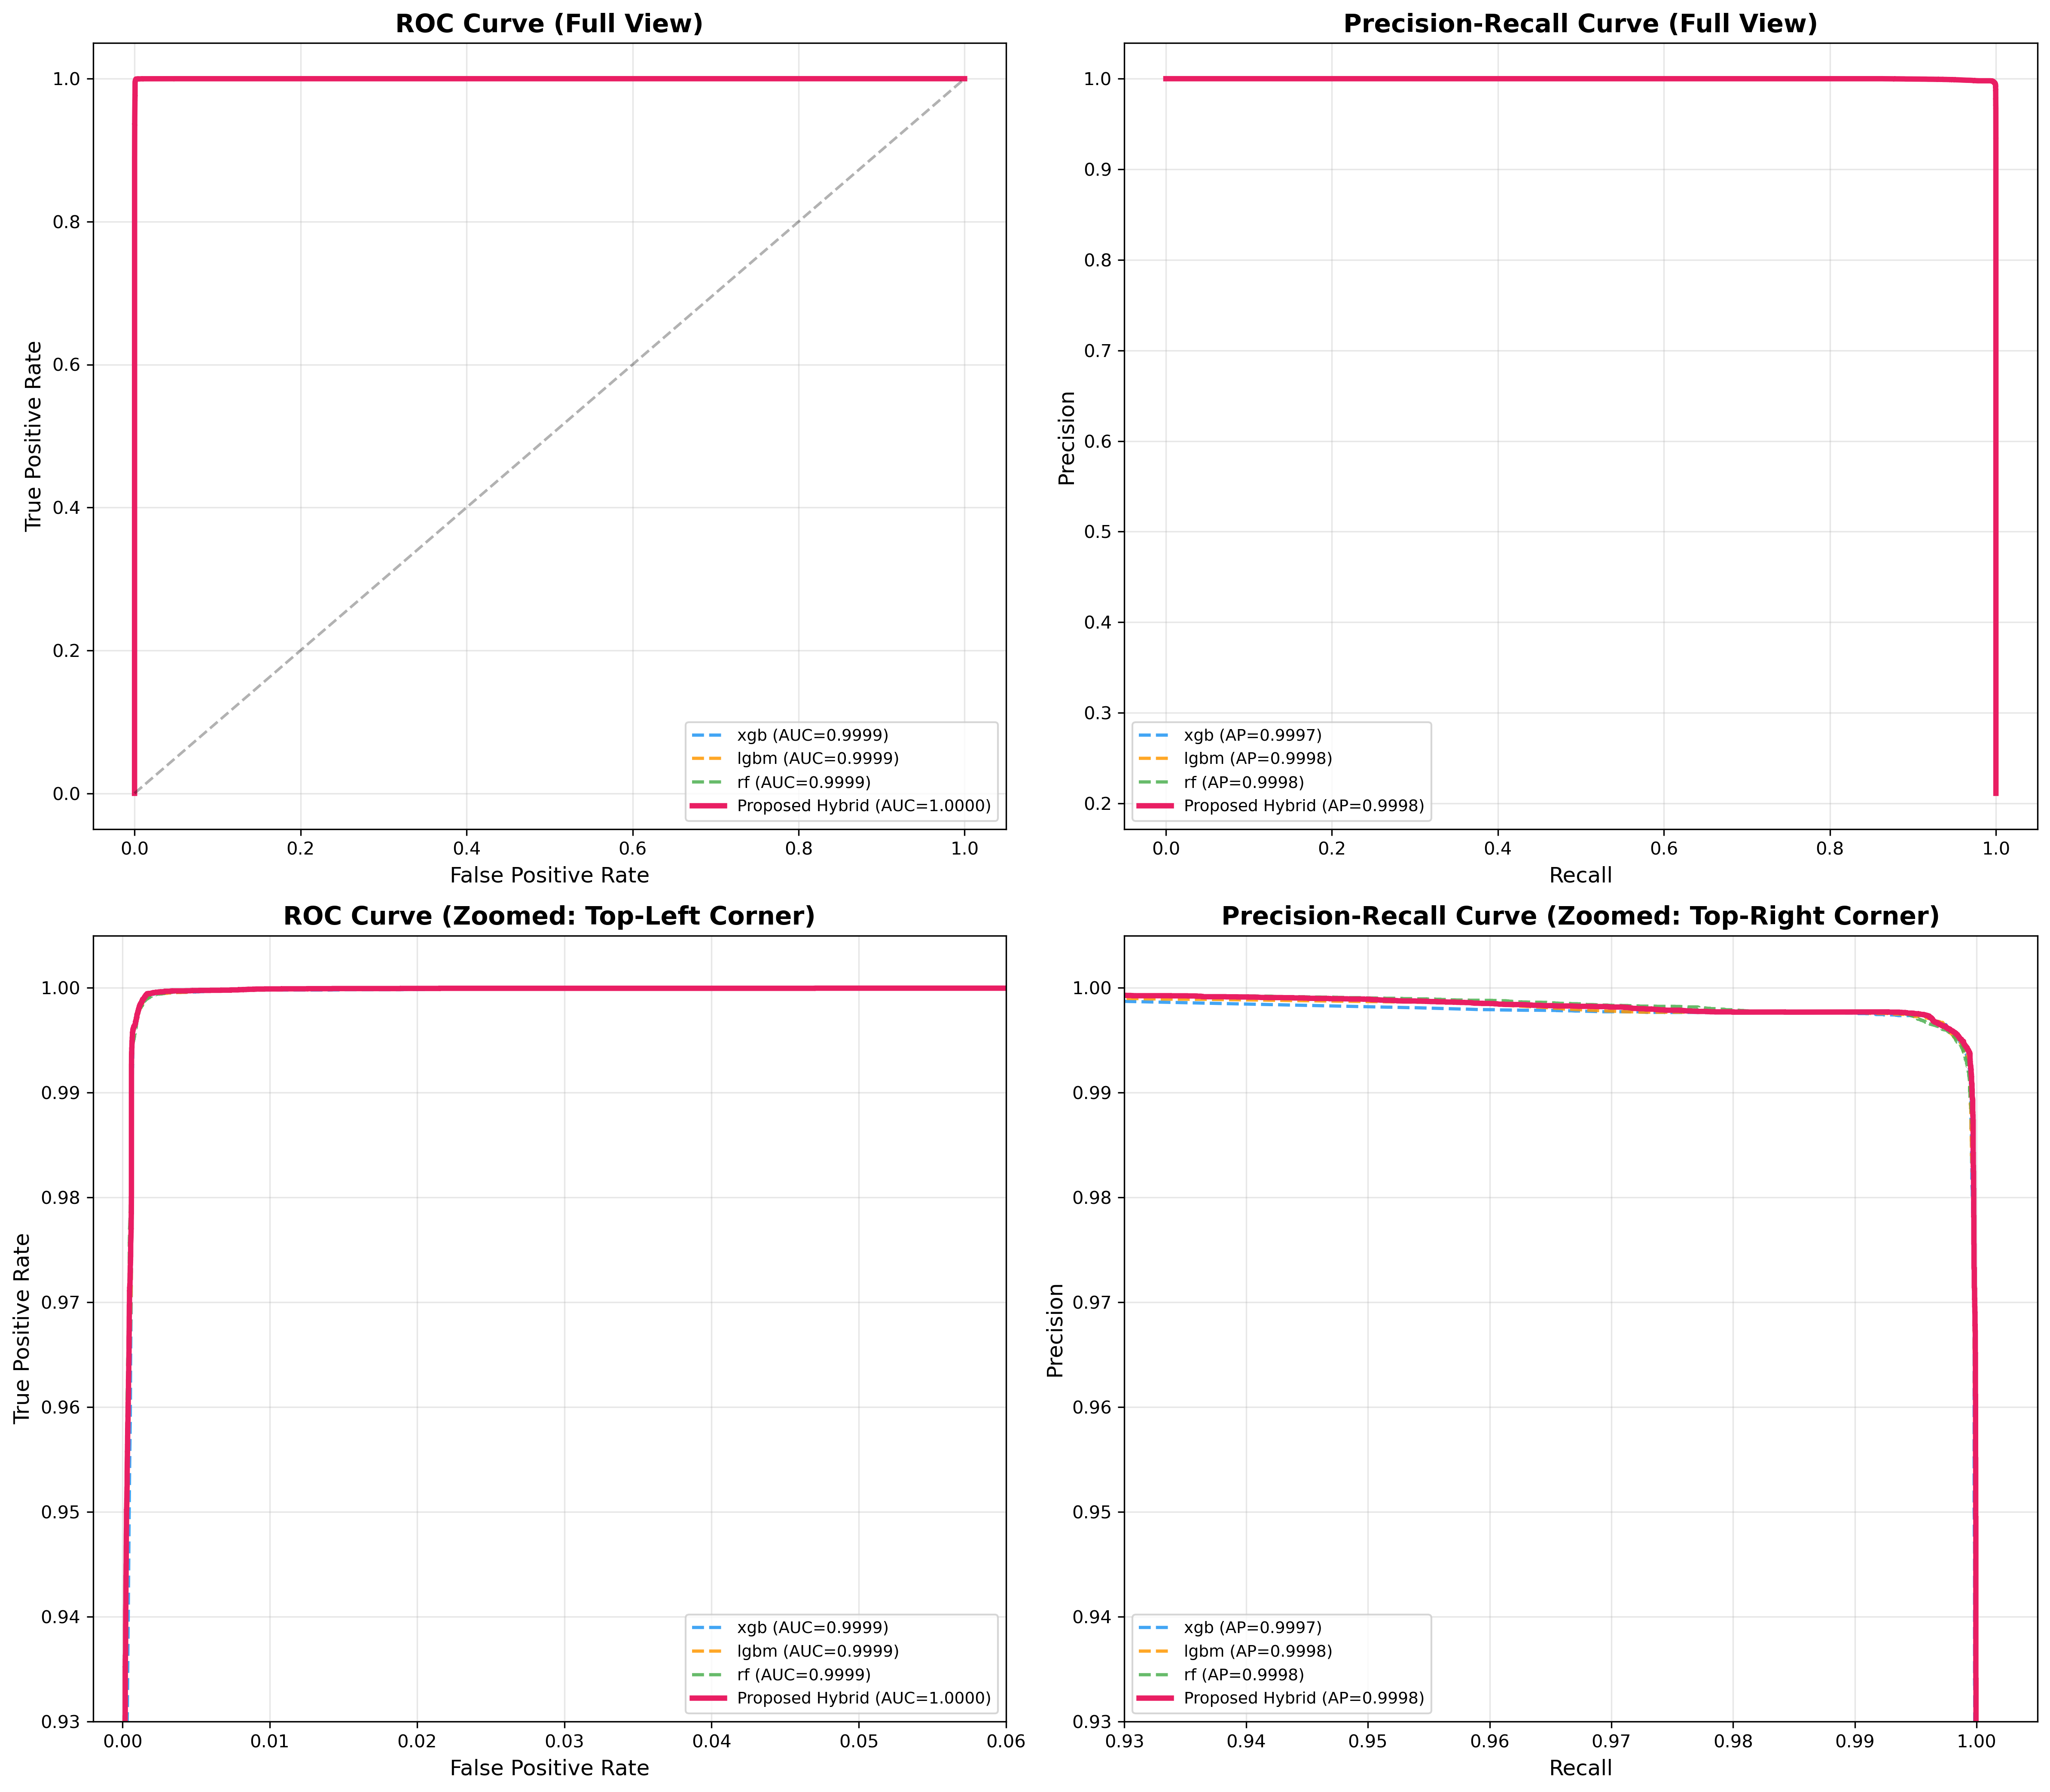
\includegraphics[width=\columnwidth]{figures/roc_pr_curves.png}
\caption{Đường cong Đặc tính hoạt động của bộ thu (ROC) và Precision-Recall (PR) cho tất cả các mô hình. Bên trái: Đường cong ROC với giá trị AUC. Bên phải: Đường cong Precision-Recall với giá trị Average Precision (AP).}
\label{fig:roc_pr}
\end{figure}

\subsection{Phân tích AUC-ROC và AUC-PR}
Hình~\ref{fig:roc_pr} trình bày các đường cong ROC và Precision-Recall cho tất cả các mô hình. Chỉ số AUC-ROC đánh giá khả năng phân loại không phụ thuộc vào ngưỡng, trong khi AUC-PR đặc biệt hữu ích cho các bộ dữ liệu mất cân bằng vì nó đo lường trực tiếp chất lượng dự đoán của lớp dương tính (tấn công).

Trong phát hiện xâm nhập, chỉ số AUC-PR cao có ý nghĩa hơn AUC-ROC vì bộ dữ liệu bị chi phối bởi lưu lượng lành tính. Một mô hình có AUC-ROC cao nhưng AUC-PR thấp vẫn có thể tạo ra số lượng cảnh báo giả không thể chấp nhận được so với số lượng nhỏ các cuộc tấn công thực tế.

\subsection{Giảm thiểu cảnh báo giả}
Trong các triển khai phát hiện xâm nhập thực tế, tỷ lệ Dương tính giả (FPR) cao gây ra tình trạng mệt mỏi do cảnh báo, khiến IDS không thể vận hành hiệu quả. Sự kết hợp giữa chiến lược lấy mẫu cân bằng (giúp làm rõ ranh giới giữa lưu lượng lành tính và tấn công) và bộ phân loại meta stacking (giúp giải quyết các trường hợp biên mơ hồ do các mô hình dựa trên cây tạo ra) được kỳ vọng sẽ mang lại tỷ lệ FPR vĩ mô thấp.

\begin{figure}[htbp]
\centering
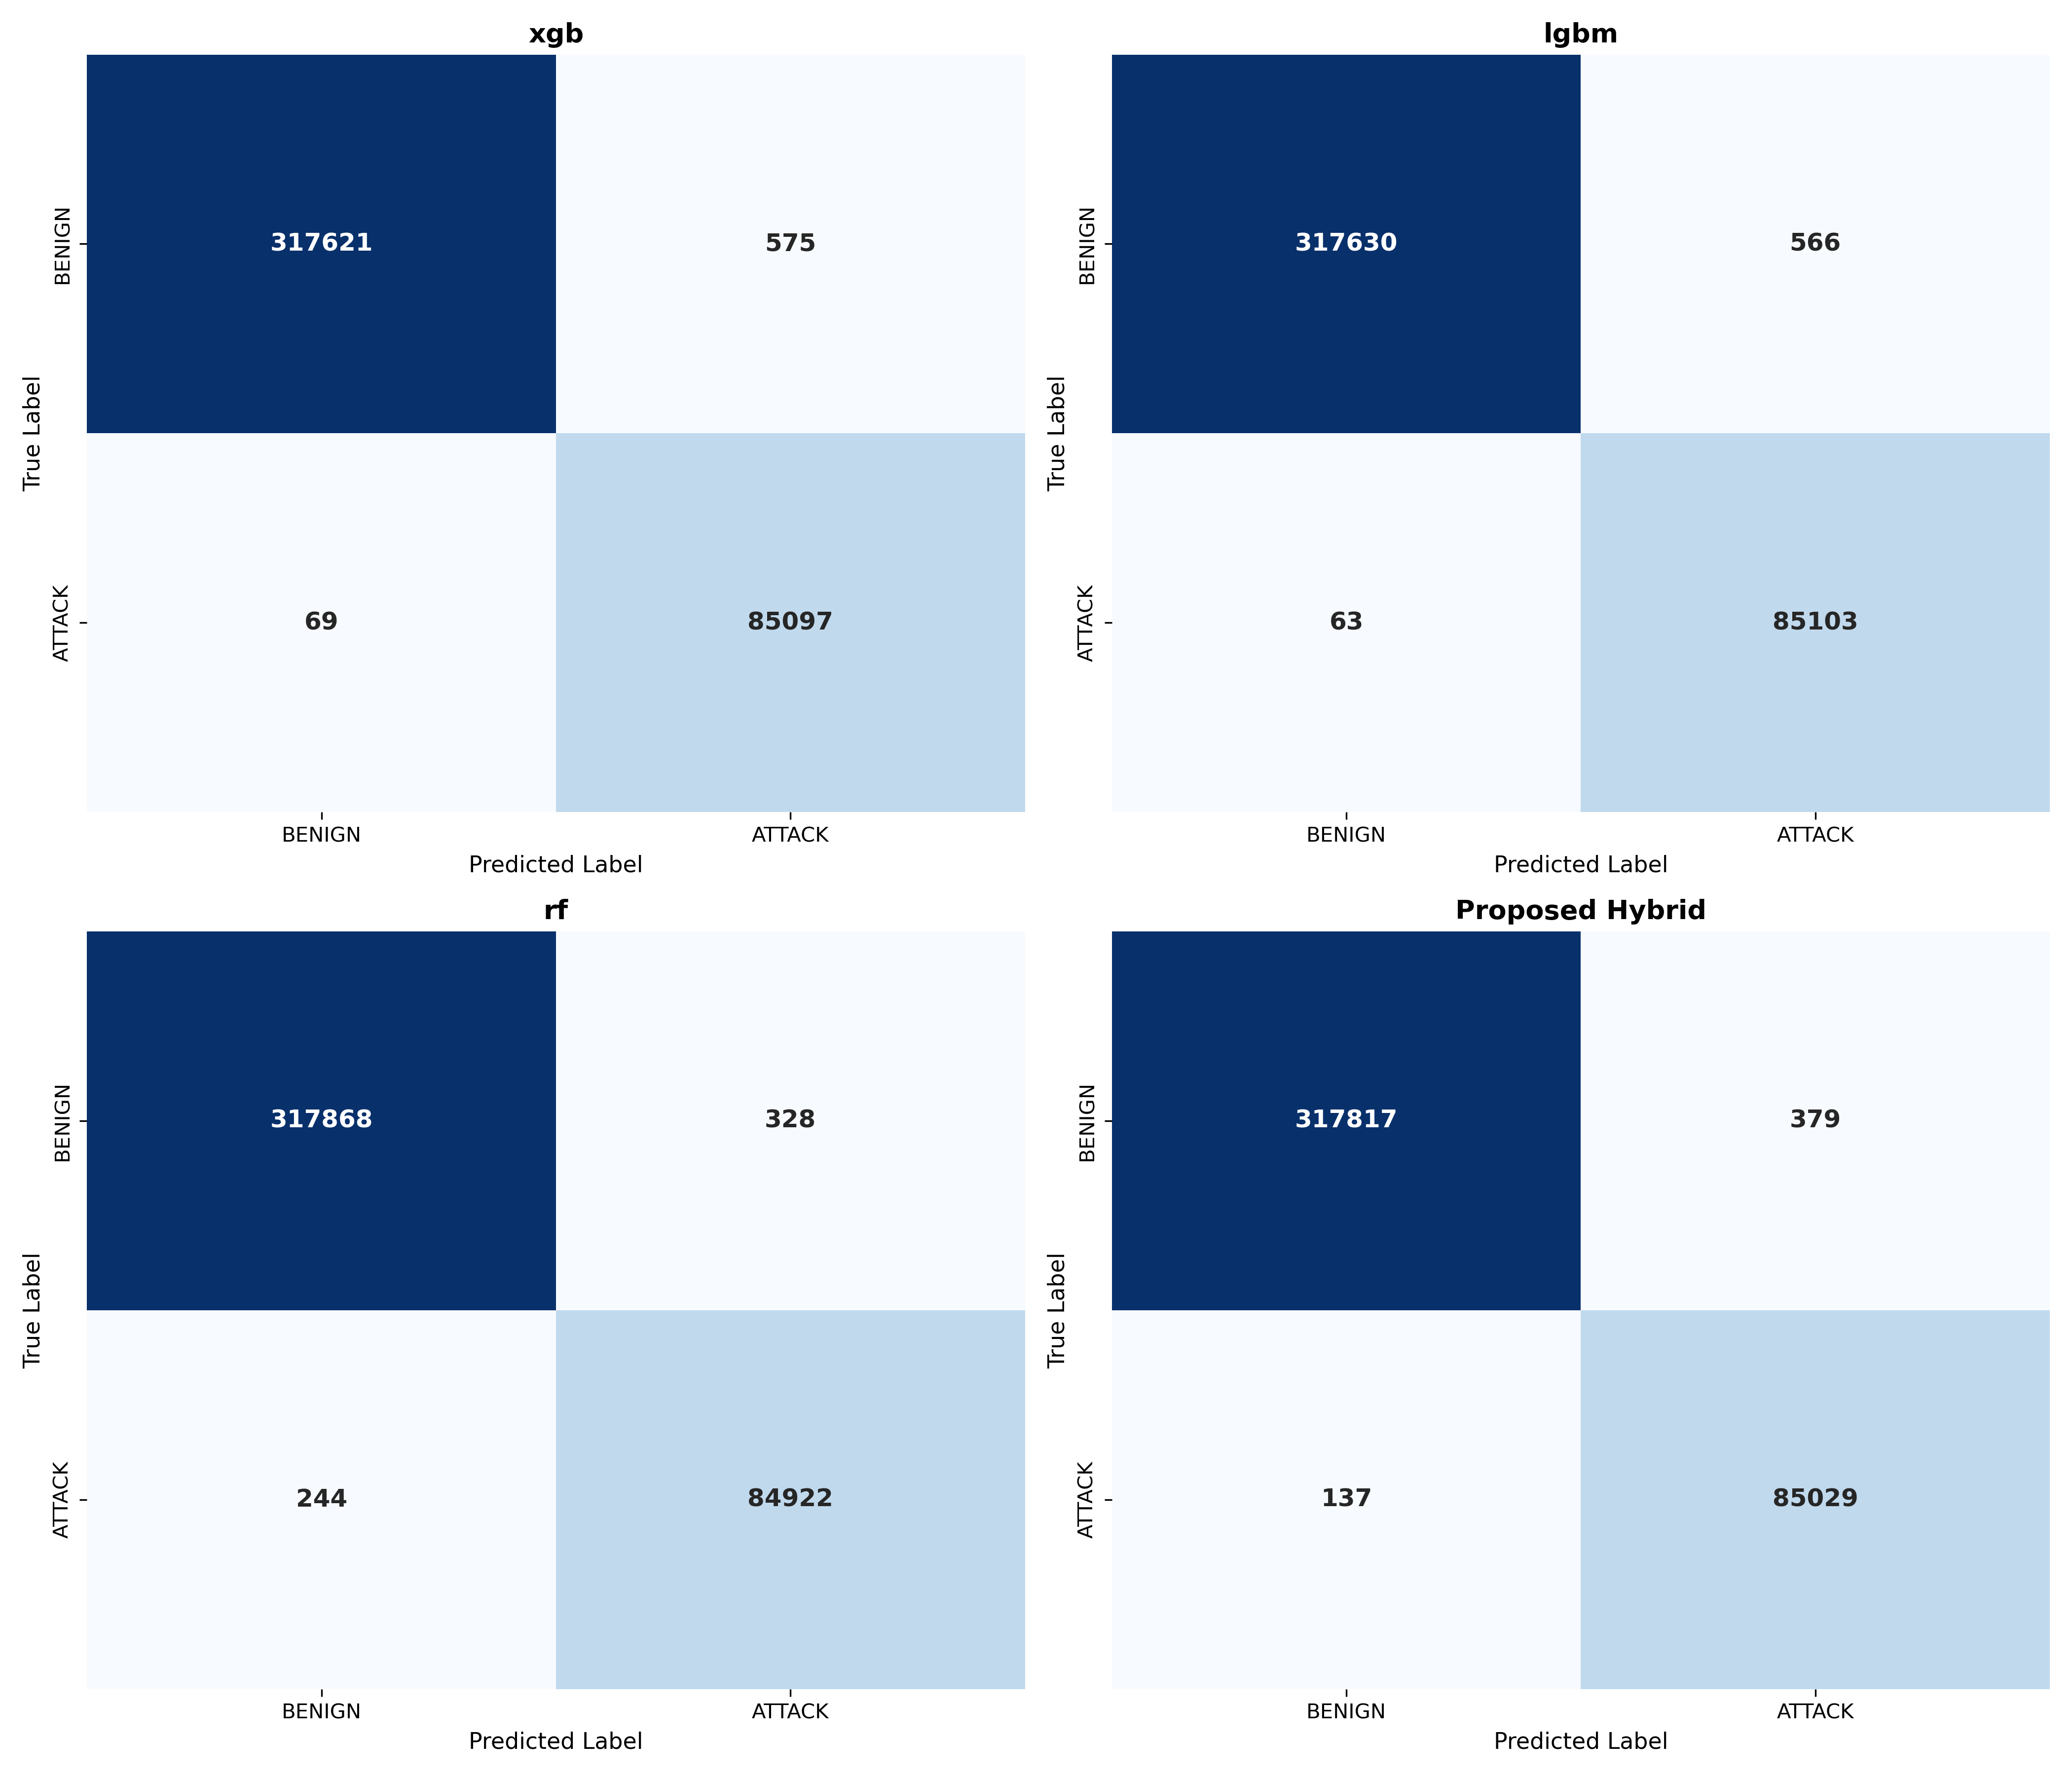
\includegraphics[width=\columnwidth]{figures/confusion_matrices.png}
\caption{Ma trận nhầm lẫn so sánh các mô hình đơn lẻ và mô hình Ensemble lai đề xuất.}
\label{fig:cm}
\end{figure}

\subsection{Phân tích tầm quan trọng của các đặc trưng}
Hiểu được các đặc trưng lưu lượng mạng nào thúc đẩy quyết định phát hiện là tối quan trọng đối với cả tính giải thích được của mô hình và triển khai thực tế. Hình~\ref{fig:feature_importance} trình bày 20 đặc trưng quan trọng nhất được trích xuất từ cả ba bộ phân loại cơ sở dựa trên cây.

\begin{figure}[htbp]
\centering
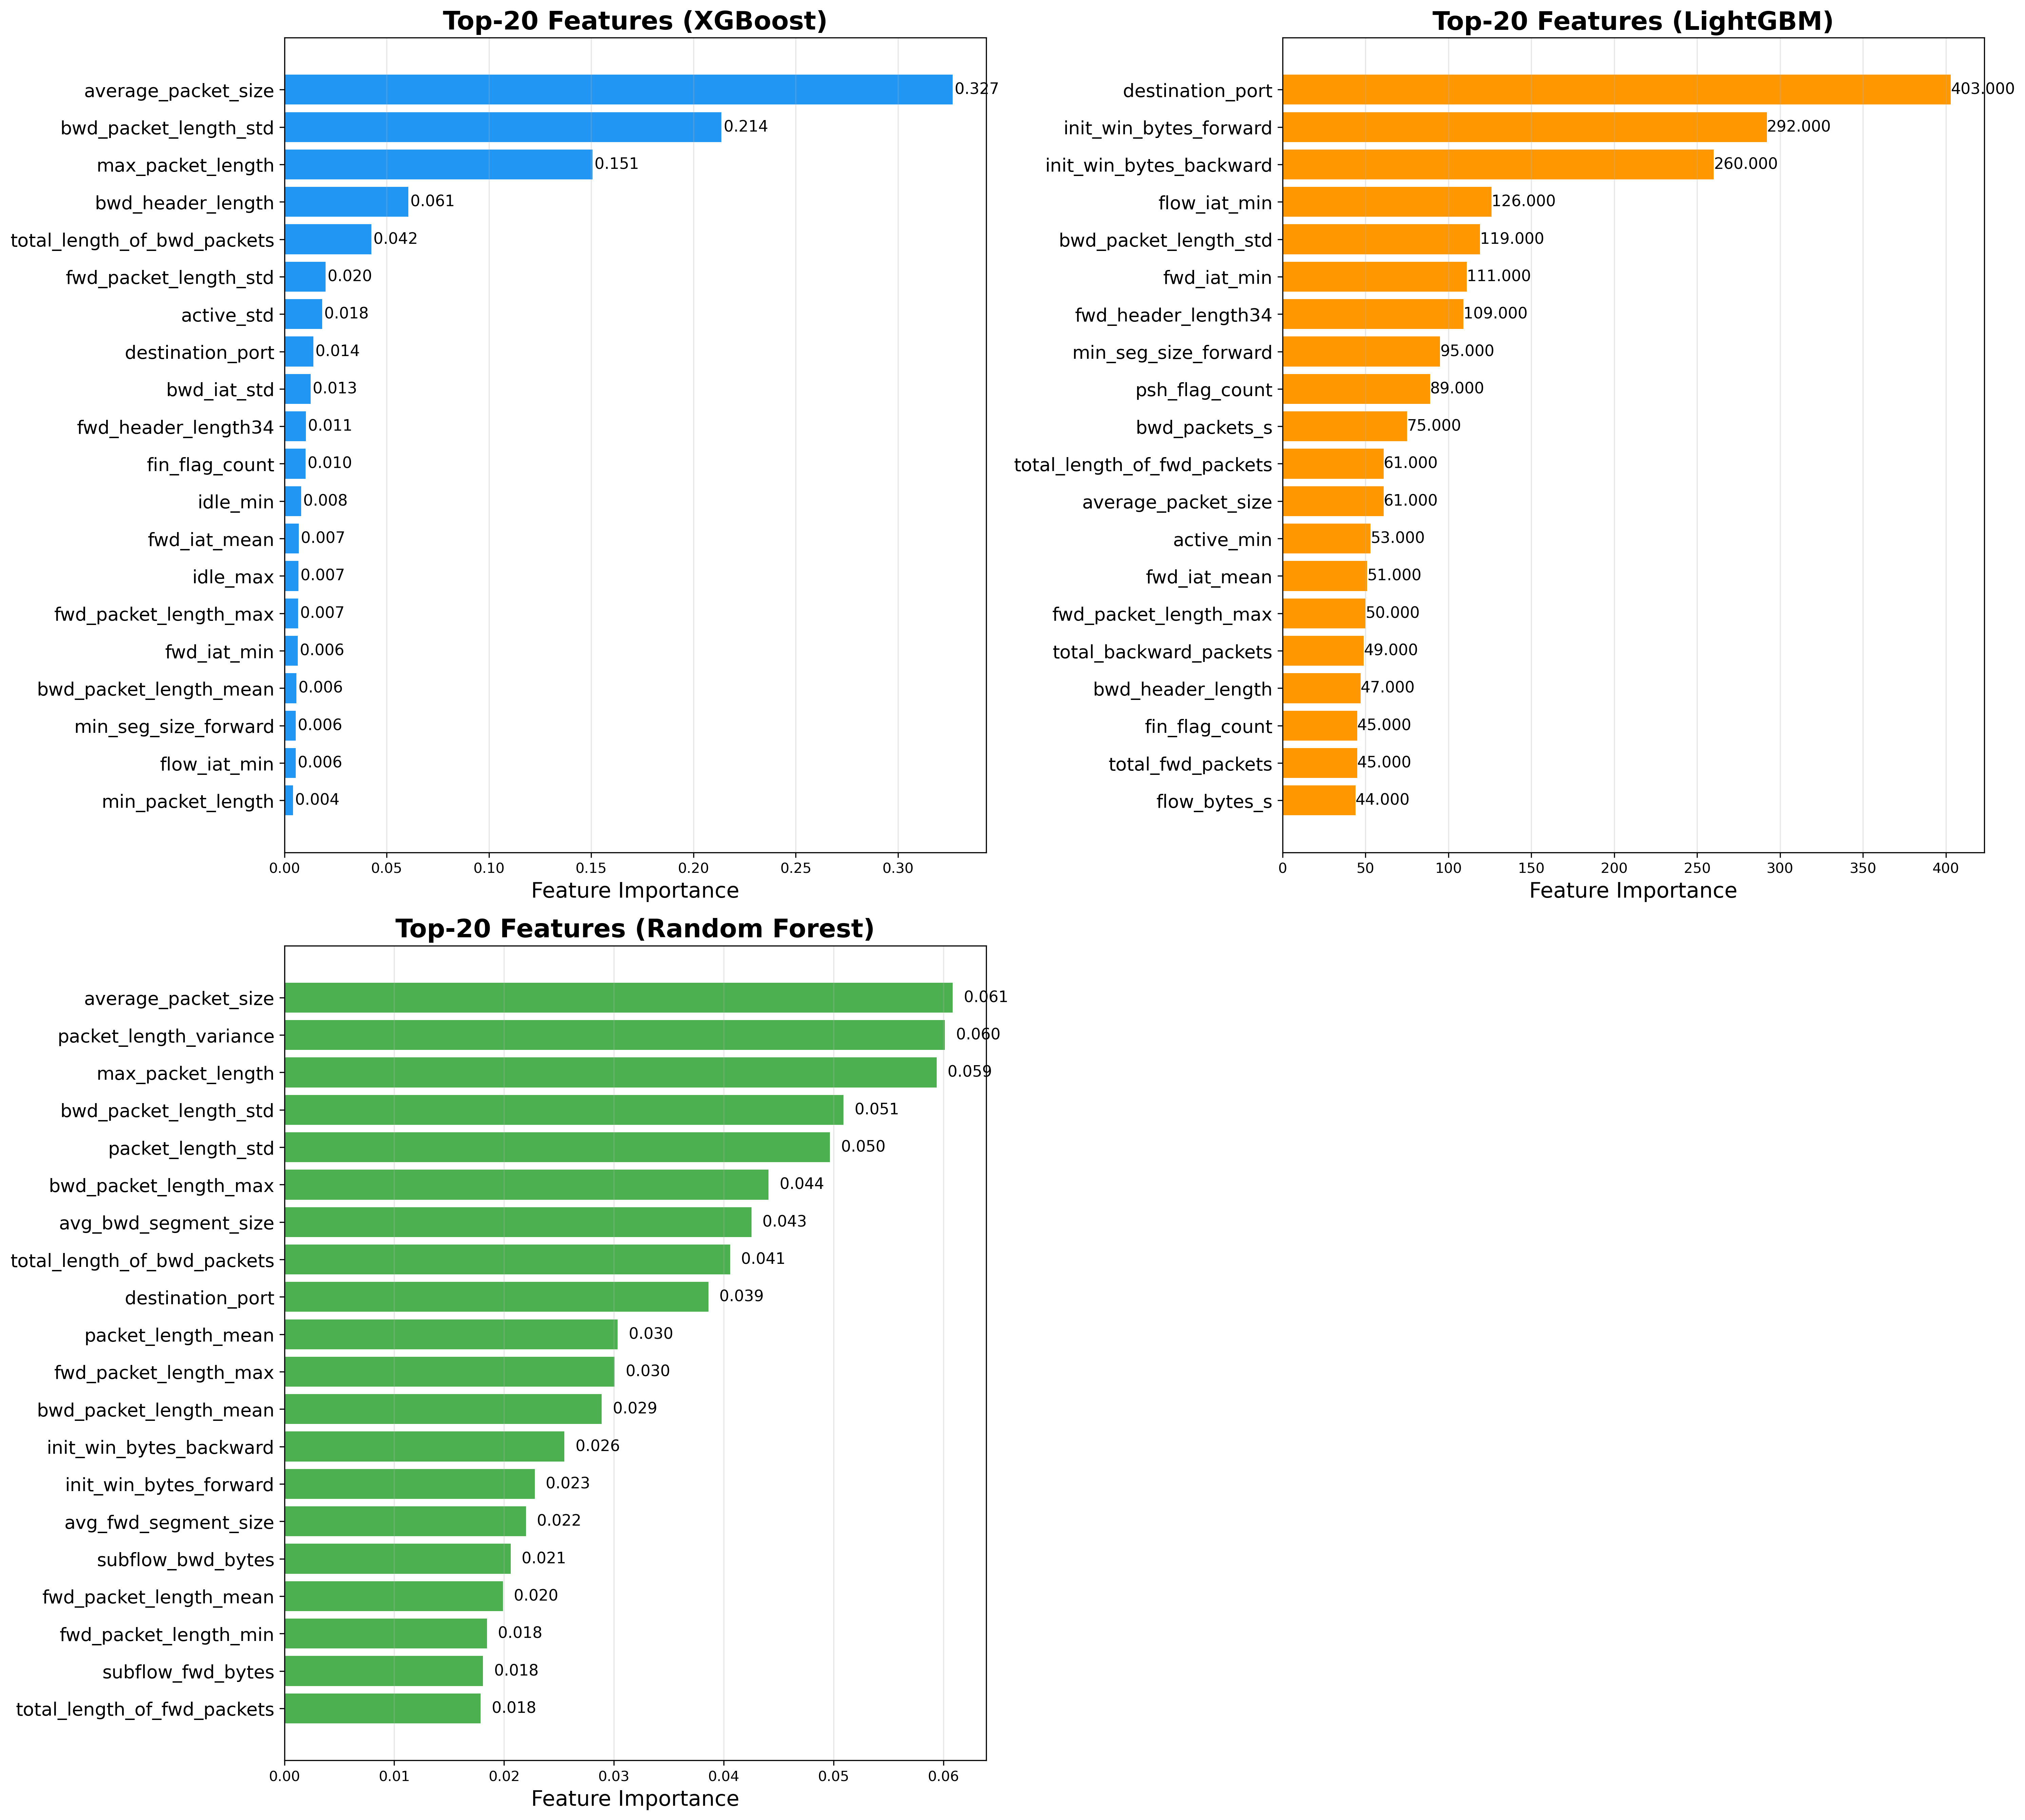
\includegraphics[width=\columnwidth]{figures/feature_importance.png}
\caption{Xếp hạng 20 đặc trưng quan trọng nhất từ các bộ phân loại cơ sở XGBoost (trái), LightGBM (giữa) và Random Forest (phải).}
\label{fig:feature_importance}
\end{figure}

Phân tích này tiết lộ các đặc điểm luồng mạng nào (ví dụ: thống kê độ dài gói tin, các phép đo thời gian luồng, số lượng cờ - flag) đóng góp nhiều nhất vào quyết định phát hiện, cung cấp những hiểu biết thực tế cho các chuyên gia an ninh mạng.

\subsection{Nghiên cứu cắt bỏ}
Để định lượng đóng góp của từng thành phần trong khung giải pháp, chúng tôi thực hiện một nghiên cứu cắt bỏ (ablation study) hệ thống. Bảng~\ref{tab:ablation} trình bày kết quả của bốn thực nghiệm.

\begin{table}[htbp]
\centering
\caption{Kết quả nghiên cứu cắt bỏ}
\label{tab:ablation}
\begin{tabularx}{\columnwidth}{@{}Xcccc@{}}
\toprule
\textbf{Cấu hình} & \textbf{Acc.} & \textbf{F1} & \textbf{FPR} & \textbf{AUC-ROC} \\
\midrule
Stacking (Không SM)              & 0,9990 & 0,9976 & 0,000861 & 0,9999    \\
Soft Voting (Có SM)              & 0,9987 & 0,9969 & 0,001373 & 0,9999    \\
Stacking (XGB+LGBM)              & 0,9985 & 0,9965 & 0,001637 & 0,9999    \\
\midrule
\textbf{Lai (Đầy đủ)}            & \textbf{0,9987} & \textbf{0,9970} & \textbf{0,001191} & \textbf{0,9999} \\
\bottomrule
\end{tabularx}
\end{table}

Nghiên cứu cắt bỏ được thiết kế để chứng minh ba đóng góp chính:
\begin{enumerate}
    \item \textbf{Tác động của SMOTEENN}: So sánh giữa dòng 1 và dòng 4 cho thấy đóng góp của việc lấy mẫu cân bằng. Việc loại bỏ SMOTEENN được kỳ vọng sẽ làm tăng FPR và giảm tỷ lệ triệu hồi đối với các lớp tấn công thiểu số.
    \item \textbf{Stacking so với Soft Voting}: So sánh giữa dòng 2 và dòng 4 minh họa lợi thế của việc học các trọng số dự đoán tối ưu thông qua một bộ phân loại meta so với việc tính trung bình xác suất đơn giản.
    \item \textbf{Đóng góp của Random Forest}: So sánh giữa dòng 3 và dòng 4 chứng minh rằng việc đưa bộ phân loại dựa trên bagging (Random Forest) vào cùng với các mô hình dựa trên boosting (XGBoost, LightGBM) giúp tăng cường sự đa dạng của tập hợp, dẫn đến khả năng tổng quát hóa tốt hơn.
\end{enumerate}

\subsection{Tính ổn định của kiểm định chéo}
Thông qua Kiểm định chéo 5 lớp phân tầng (Phần V-F), chúng tôi đã chứng minh rằng khung đề xuất đạt được hiệu năng ổn định trên các phân vùng dữ liệu khác nhau. Độ lệch chuẩn thấp xác nhận rằng kết quả của chúng tôi đạt được không phải do sự may mắn từ một lần chia tập huấn luyện/kiểm tra thuận lợi, cung cấp bằng chứng mạnh mẽ về khả năng tổng quát hóa.

\begin{figure}[htbp]
\centering
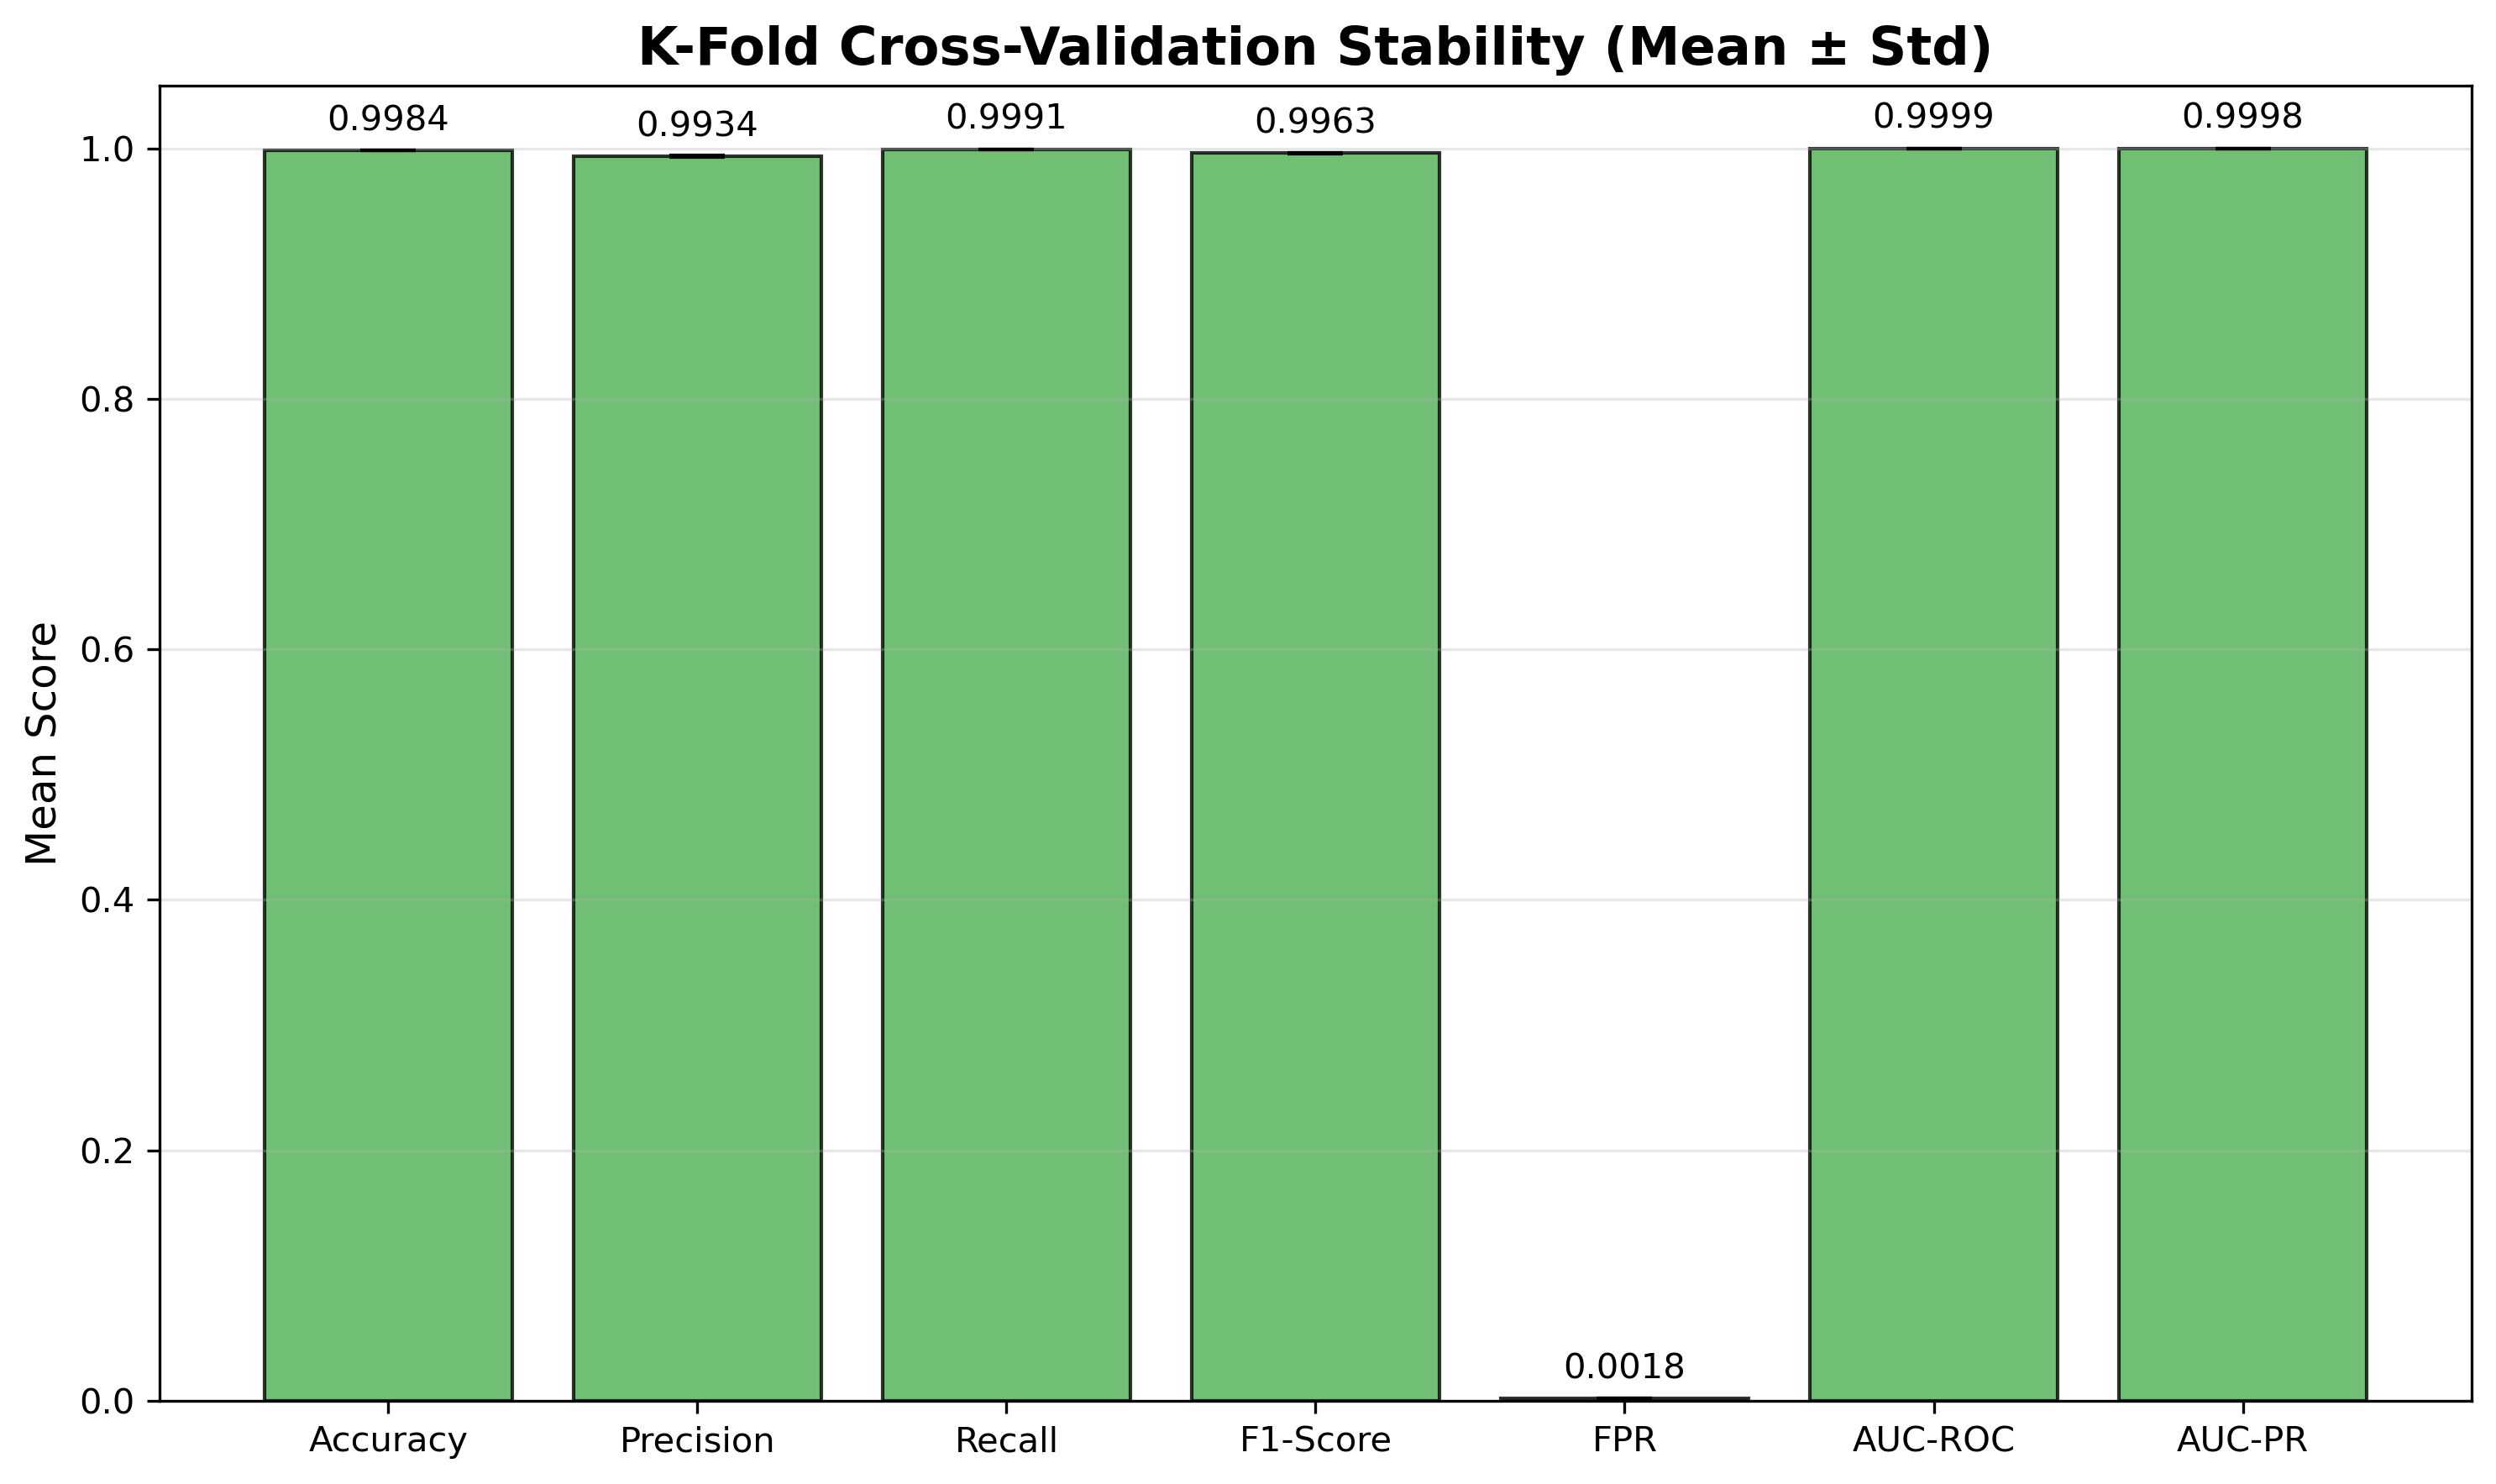
\includegraphics[width=\columnwidth]{figures/cv_stability.png}
\caption{Tính ổn định về hiệu năng của mô hình Ensemble lai qua 5 lớp phân tầng, chứng minh khả năng tổng quát hóa mạnh mẽ với độ lệch chuẩn không đáng kể.}
\label{fig:cv_stability}
\end{figure}

Bảng~\ref{tab:cv_results} tóm tắt các chỉ số kiểm định chéo 5 lớp.

\begin{table}[htbp]
\centering
\caption{Kết quả Kiểm định chéo 5 lớp phân tầng (Trung bình $\pm$ Độ lệch chuẩn)}
\label{tab:cv_results}
\begin{tabular*}{\columnwidth}{@{\extracolsep{\fill}}lc@{}}
\toprule
\textbf{Chỉ số} & \textbf{Trung bình $\pm$ Độ lệch chuẩn} \\
\midrule
Accuracy     & $0,9984 \pm 0,000131$ \\
Precision    & $0,9934 \pm 0,000611$ \\
Recall       & $0,9991 \pm 0,000106$ \\
F1-Score     & $0,9963 \pm 0,000309$ \\
FPR          & $0,0018 \pm 0,000165$ \\
AUC-ROC      & $0,9999 \pm 0,000004$ \\
AUC-PR       & $0,9998 \pm 0,000010$ \\
\bottomrule
\end{tabular*}
\end{table}

Các giá trị độ lệch chuẩn thấp trên các lớp kiểm định xác nhận rằng khung đề xuất có khả năng tổng quát hóa tốt và hiệu năng của nó là ổn định bất kể sự phân chia dữ liệu cụ thể nào, từ đó xác nhận tính mạnh mẽ của phương pháp tiếp cận của chúng tôi.

\subsection{So sánh với các nghiên cứu gần đây}
Để làm nổi bật hiệu năng của khung đề xuất, Bảng~\ref{tab:literature_comparison} so sánh kết quả của chúng tôi với các nghiên cứu hiện đại gần đây (2024--2026) cũng thực hiện đánh giá trên bộ dữ liệu CICIDS2017 với phân loại nhị phân.

\begin{table}[htbp]
\centering
\caption{So sánh với các nghiên cứu gần đây trên CICIDS2017 (2024--2026)}
\label{tab:literature_comparison}
\begin{tabularx}{\columnwidth}{@{}p{2.8cm}Xcc@{}}
\toprule
\textbf{Nghiên cứu} & \textbf{Phương pháp} & \textbf{Acc. (\%)} & \textbf{F1 (\%)} \\
\midrule
Amara et al. (2025) \cite{amara2025stacked}     & CNN+TCN+LSTM Ens.     & 99,99 & 100,0 \\
Nguyen et al. (2024) \cite{nguyen2024apelid}     & Augmented WGAN + Ens. & 99,78 & --    \\
Ding et al. (2024) \cite{ding2024tmg}      & TMG-GAN + DNN         & 99,81 & 99,72 \\
Khan et al. (2024) \cite{khan2024balanced}      & SMOTE-Tomek + DT      & 99,96 & --    \\
Hu et al. (2024) \cite{hu2024improved}        & Hybrid Attention      & 99,79 & --    \\
Ji (2025) \cite{ji2025hybrid}             & GRU-ResCBANet         & 99,83 & --    \\
Sarhan et al. (2022) \cite{sarhan2022towards}    & ML Baseline (TII)     & 99,70 & 99,20 \\
\midrule
\textbf{Đề xuất}     & \textbf{Hybrid Ensemble} & \textbf{99,87} & \textbf{99,70} \\
\bottomrule
\end{tabularx}
\vspace{2pt}
\footnotesize{\textit{Ghi chú: ``--'' cho biết chỉ số không được báo cáo cụ thể trong nghiên cứu gốc.}}
\end{table}

Như được trình bày trong Bảng~\ref{tab:literature_comparison}, mô hình Ensemble lai đề xuất của chúng tôi đạt được hiệu năng cạnh tranh với các phương pháp hiện đại gần đây, bao gồm cả các nghiên cứu rất mới từ năm 2025. Trong khi các kiến thuật cụ thể phức tạp như DL ensemble xếp chồng của Amara và cộng sự \cite{amara2025stacked} đạt được điểm số gần 100\%, chúng dựa trên các thành phần tốn kém tài nguyên tính toán (CNN, TCN, LSTM) thường gây khó khăn cho việc triển khai tại biên. Khung giải pháp của chúng tôi đạt được sự cân bằng tối ưu giữa hiệu năng phát hiện cao và độ phức tạp tính toán thấp. Bằng việc đạt được Độ chính xác 99,87\% và điểm F1 99,70\% thông qua bộ ensemble dựa trên cây đa dạng, cùng với việc nén thêm qua kỹ thuật Chưng cất tri thức (Bảng~\ref{tab:kd_results}), chúng tôi cung cấp một giải pháp mạnh mẽ và có khả năng tổng quát hóa cao, được tối ưu hóa đặc biệt cho các môi trường biên thời gian thực với yêu cầu độ trễ dưới một phần nghìn giây.

\subsection{Hiệu quả suy luận và Chưng cất tri thức}
Đối với việc triển khai thực tế trong các cổng IoT và thiết bị điện toán Biên, độ chính xác của mô hình phải được cân bằng cẩn thận với độ trễ suy luận. Để chứng minh tính linh hoạt trong vận hành của khung giải pháp, chúng tôi đã áp dụng kỹ thuật Chưng cất kiến thức (Phần III-D). Mô hình Ensemble lai đồ sộ (Teacher) đã được nén thành một Cây Quyết định nhẹ (Student).

\begin{figure}[htbp]
\centering

\includegraphics[width=\columnwidth]{figures/inference_tradeoff.png}
\caption{Sự đánh đổi về Độ chính xác và Tốc độ suy luận giữa mô hình Ensemble lai (Teacher) và Cây quyết định đã được chưng cất (Student). Lưu ý thang đo logarit cho thời gian suy luận.}
\label{fig:kd_tradeoff}
\end{figure}

Bảng~\ref{tab:kd_results} trình bày sự so sánh về hiệu năng và độ trễ (đo bằng mili giây trên 1.000 mẫu).

\begin{table}[htbp]
\centering
\caption{Chưng cất tri thức: Hiệu năng so với Dấu ấn triển khai}
\label{tab:kd_results}
\begin{tabularx}{\columnwidth}{@{}lXXcc@{}}
\toprule
\textbf{Mô hình} & \textbf{Acc.} & \textbf{F1} & \textbf{Inf. (ms/1k)} & \textbf{Bộ nhớ (MB)} \\
\midrule
Teacher (Ens.)     & 0,9987 & 0,9970 & 2,25 & 36,24 \\
Student (DT)       & 0,9965 & 0,9918 & 0,09 & 0,0244 \\
\bottomrule
\end{tabularx}
\end{table}

Mô hình Student sau khi chưng cất vẫn duy trì được phần lớn khả năng phát hiện của Teacher trong khi đạt được sự giảm thiểu khổng lồ về cả độ trễ suy luận và dung lượng bộ nhớ. Điều này xác nhận rằng các ranh giới quyết định phức tạp mà mô hình Ensemble lai đã học được có thể chuyển giao hiệu quả sang một kiến trúc bị giới hạn về tính toán thông qua kỹ thuật chưng cất tri thức, cung cấp một giải pháp có khả năng mở rộng cao cho các Hệ thống Phát hiện Xâm nhập dựa trên biên với yêu cầu độ trễ dưới một phần nghìn giây.
